\documentclass{beamer}
\usepackage[latin1]{inputenc}
%\usetheme[noshadow,nonav,nologo]{NYU}
\usetheme[numbers]{NYU}
\usepackage{amsmath}
\usepackage{amsfonts}
\usepackage{amssymb}
\usepackage{color, colortbl}

\makeatletter
\newcommand{\thickhline}{%
    \noalign {\ifnum 0=`}\fi \hrule height 2pt
    \futurelet \reserved@a \@xhline}

\title{Representation of High Dimensional Data}
\date{October 30, 2012} 
\author{Ross Goroshin}

\begin{document}

\begin{frame}
\titlepage
\end{frame}

\begin{frame}
\frametitle{Dimensionality of Data \& Statistical Dependence}  
\begin{center}
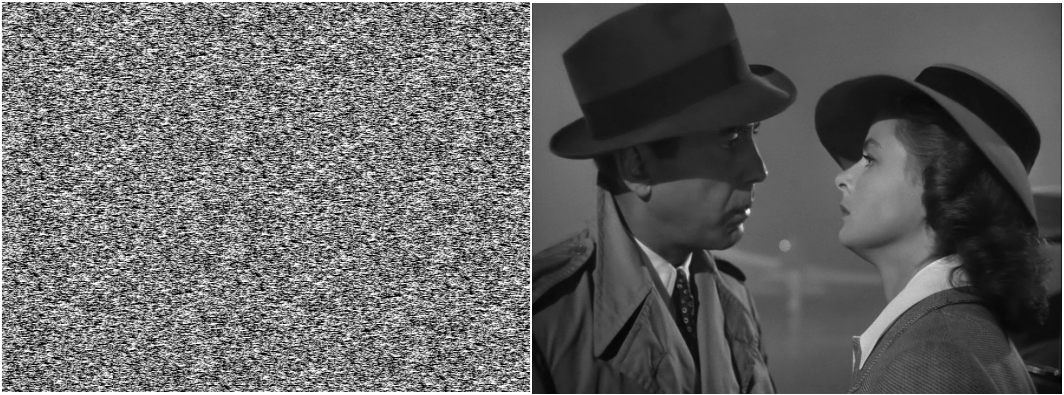
\includegraphics[scale=0.125]{image.png}
\begin{itemize} 
\item Suppose we have a 42 second video played at 24 frames/second, with a resolution of 1000 by 1000 pixels
\item In theory each pixel can vary independently from frame to frame, which implies that there are $\approx 10^9$ degrees of freedom 
\item If all of these pixels were to vary independently of one another, the picture would not be very interesting
\item Moreover if you were to describe the content of the video to a friend over the telephone, it is doubtful that the term 'pixel' would ever be mentioned in the conversation 
\end{itemize} 
\end{center}
\end{frame}

\begin{frame} 
\frametitle{Dimensionality of Data \& Statistical Dependence}
\begin{center} 
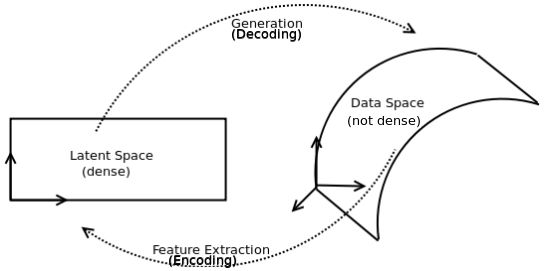
\includegraphics[scale = 0.5]{spaces.png}
\end{center} 
\begin{itemize} 
\item This illustration is representative of many processes 
\item However, dependence can be introduced without increasing the dimensionality 
\item Latent representation is NOT unique for generative processes of interest
\end{itemize}  
\end{frame}

\begin{frame}
\small
\frametitle{Relationship Between Approaches} 
\begin{tabular}{c||c|c|c|c}
Algorithm & Model & Encode & Decode & Relate Enc. \& Dec.\\
\thickhline
\cellcolor{red}PCA & Global Linear &\checkmark & \checkmark & $W_D = W_E ^T$\\
\hline
\cellcolor{red}ICA & Global Linear &\checkmark & \checkmark & $W_D = W_E ^T$\\
\thickhline
\cellcolor{yellow}Sparse Coding & Local Linear &\checkmark(\$) & \checkmark & $W_D = W_E ^T$ \\
\hline 
\cellcolor{yellow}PSD \& LISTA & Local Linear &\checkmark & \checkmark & Learned $W_E$\\
\hline
\cellcolor{orange}DrLIM & Nonlinear & \checkmark & X & Enc. Only\\
\hline
\cellcolor{green}Auto-Encoders & Nonlinear & \checkmark & \checkmark & Learned $W_E$ \& $W_D$ 
\end{tabular} \\
\begin{center}
\begin{tabular}{c|c|}
\hline
\cellcolor{red} \hspace{10 mm} & De-correlation/Independence  \\
\cellcolor{yellow} \hspace{10 mm} & Sparsity \\
\hline
\cellcolor{orange} \hspace{10 mm} & Metric Learning/Restricted Metric Learning  \\
\hline
\cellcolor{green} \hspace{10 mm} & All of the Above \\
\hline
\end{tabular}
\end{center} 
\end{frame} 


\begin{frame} 
\frametitle{First Attempt at Independence: PCA} 
\begin{itemize} 
\item Assume you have $x = As$ where each $x_i \in \mathbb{R}^D$ ($s$ blue, $x$ red)
\item PCA assumes that there are $M \leq D$ linearly interdependent combinations of the input space variables which are responsible for most of the variance of the data 
\end{itemize}
\begin{equation} 
\nonumber
\frac{1}{N} \sum_{n=1}^N (e_1 ^T x_n - e_1 ^T \bar{x}) ^2  = e_1^T \frac{1}{N} \sum _{i=1}^N (x_i - \bar{x})(x_i-\bar{x})^T e_1
\end{equation}  
Leading to the problem: maximize $e_1^T \Sigma e_1$ s.t $e_1^T e_1 =1$ where $\Sigma$ is the covariance matrix. 
\begin{center} 
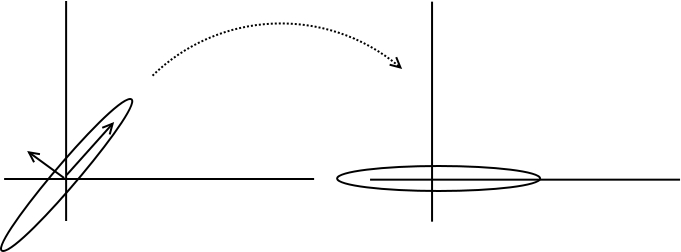
\includegraphics[scale = 0.15]{PCA.png}\\
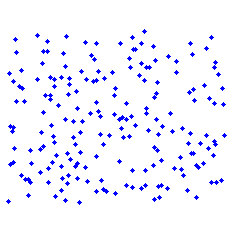
\includegraphics[scale = 0.20]{PCA2.png}
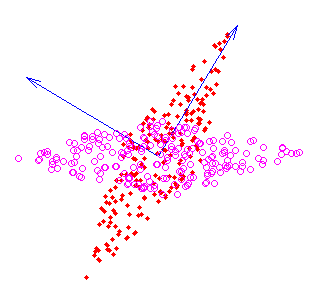
\includegraphics[scale = 0.20]{PCA3.png}
\end{center} 
\end{frame} 

\begin{frame}
\frametitle{Global Variations are Not Everything} 
\begin{center}
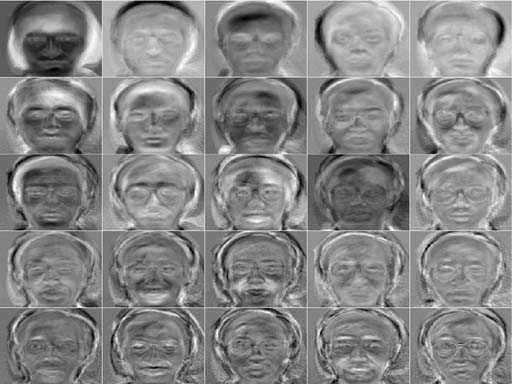
\includegraphics[scale = 0.2]{eigenfaces.jpg}
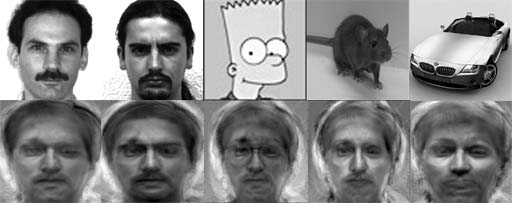
\includegraphics[scale = 0.2]{nonfaces.jpg}\\
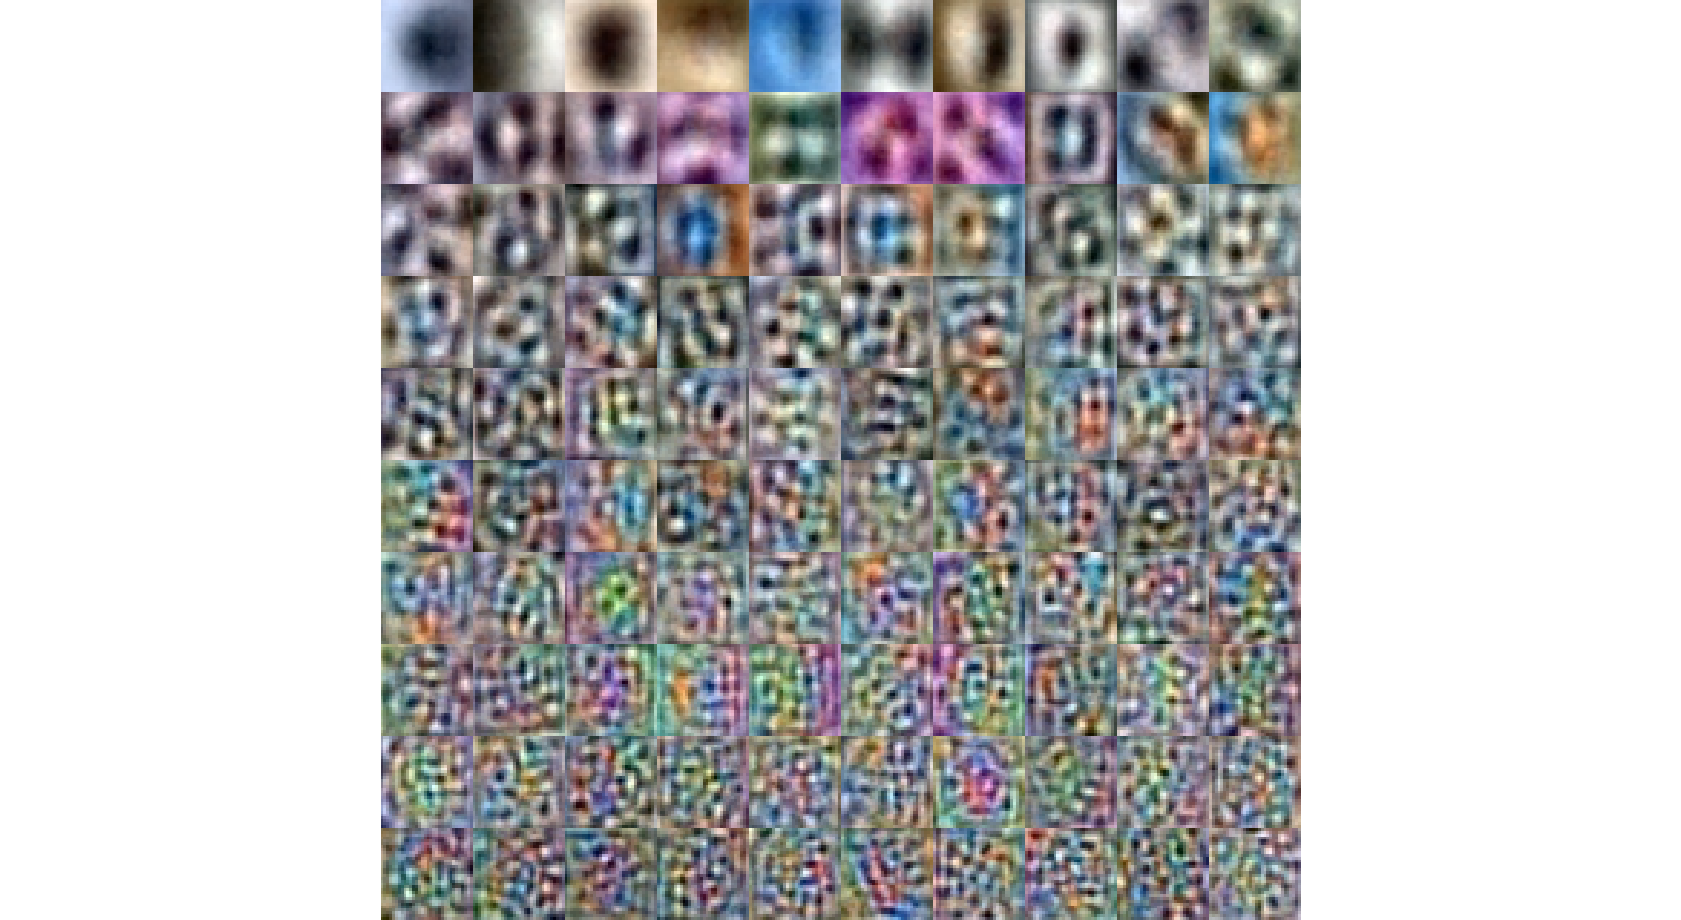
\includegraphics[scale = 0.2]{ColorPCA.png}
\end{center} 
\end{frame}

\begin{frame} 
\frametitle{A Little Closer to Independence: Whitening} 
\begin{itemize}
\item{Note that the covariance matrix of the data in PCA space is diagonal, i.e. the data is completely uncorrelated}
\item{Whitening the data is equalizing the variance of the uncorrelated data}  
\item{The whitening transform is given by $V = W D^{-1/2} W ^T$} 
\item{The whiteness property of the data is invariant to orthogonal transforms. Let $E[zz^T] = \bf I$, and let $y = Uz$ where $U$ is an orthogonal transform.} \item{Then $E[yy^T] = E[Uzz^T U^T] = U E[zz^T]U^T = \bf I$}. Whitening produces the ICs, modulo an orthogonal transform  
\end{itemize} 
For radially symmetric distributions (e.g. Gaussian) we are done! 
\begin{center}
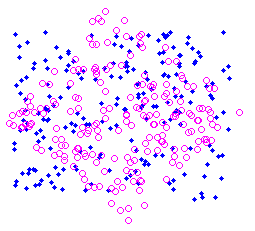
\includegraphics[scale = 0.3]{white.png}
\end{center} 
\end{frame} 

\begin{frame} 
\frametitle{Independent Component Analysis} 
\begin{itemize} 
\item{Generative model $x=As$, where neither the $A$ nor the $s$ are known. Focus on picking out one of the $s$ components at a time, i.e. $ y  = b^T A s (= q_1 s_1 + q_2 s_2$ for 2D)} 
\item{Assume that the $s$ mixture components are i.i.d and non-Gaussian, by the central limit theorem any mixture of the variables is more "Gaussian" than the individual distributions}  
\item{A good measure of non-Gaussianity is $k(y) = E[y^4] - 3(E[y^2])^2$. For whitened data, $k(y) = E[y^4] - 3$}
\item{Since the data has been whitened, we constrain $E[y^2] = q_1 ^ 2 var(s_1) + q_2^2 var(s_2) + cov(s_1,s_2) = q_1 ^ 2 + q_2 ^2 = 1$}  
\end{itemize} 
\end{frame} 

\begin{frame} 
\frametitle{Independent Component Analysis} 
\begin{itemize}
\item{max $|kurt(y)| = |q_1 ^ 4 kurt(s_1) + q_2 ^ 4kurt(s_2)|$ s.t. $q_1 ^ 2 + q_2 ^2 = 1$} 
\item{Assuming that $s_1$ and $s_2$ are i.i.d then $kurt(s_1) = kurt(s_2)$}. 
\item{However we don't directly have access to the $q$ variables (they are mixed by $A$) making it expensive to enforce the constraint $\|q\|^2 =1$. If the data is whitened however, and we seek the linear combination $w^Tz$ that maximizes non-Gaussianity then it can be show that $\|q\| = \|w\|$} 
\end{itemize}
\begin{center}
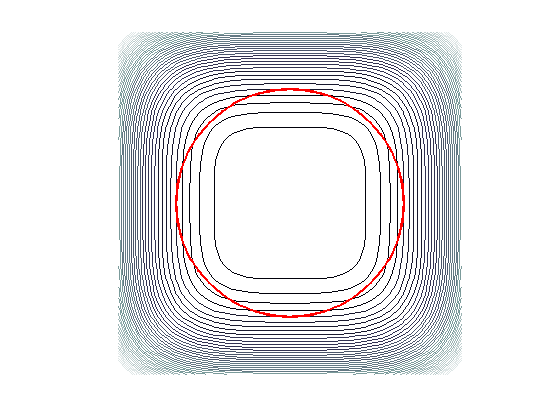
\includegraphics[scale = 0.3]{ICA.png}
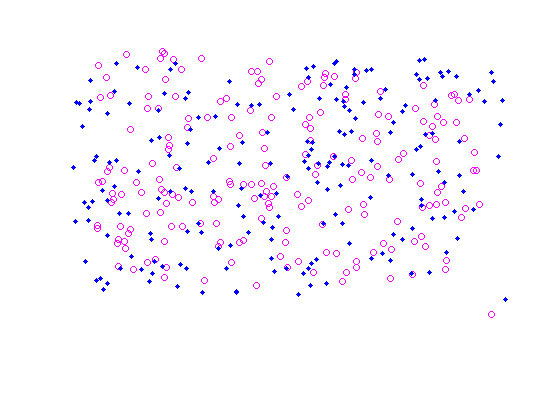
\includegraphics[scale = 0.3]{ICAresult1.png}
\end{center}
\end{frame} 

\begin{frame}
\frametitle{ICA Results}  
\begin{center}
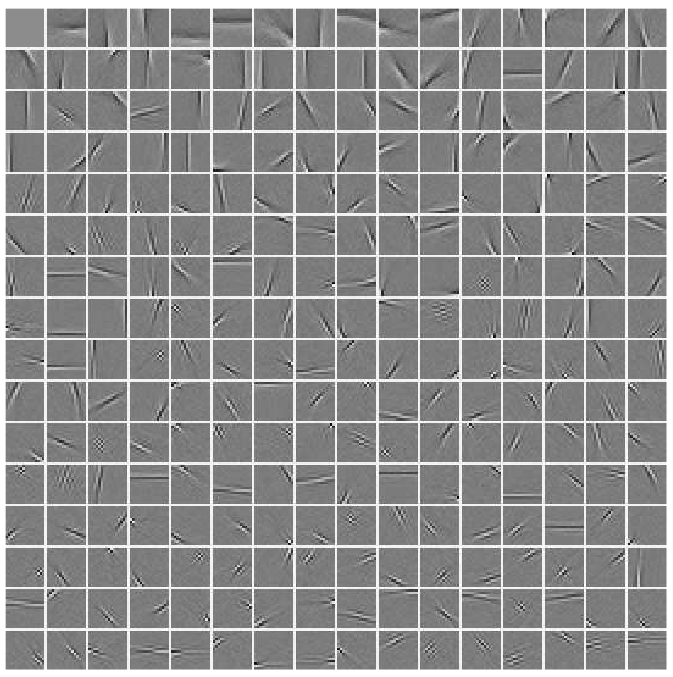
\includegraphics[scale = 0.3]{ICABasis.png}
\end{center} 
\end{frame} 

\begin{frame}
\frametitle{ICA Results}
\begin{center}
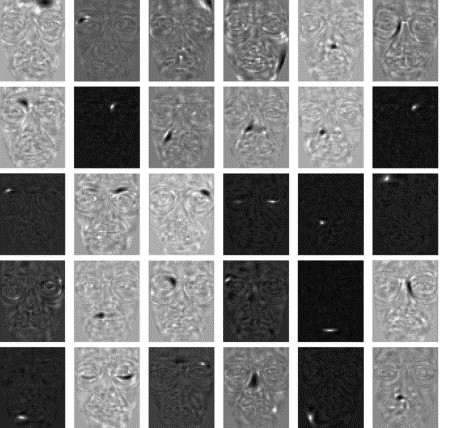
\includegraphics[scale = 0.5]{ICAfaces.jpg}
\end{center} 
\begin{itemize}
\item{Note that vectors found by ICA are more localized, i.e. individual activations are sparsely distributed (super-Gaussian) over the data}  
\end{itemize} 
\end{frame} 

\begin{frame}
\frametitle{Limit of Classical ICA} 
The $x=As$ model is invalid for nonlinear data manifolds
\begin{center}
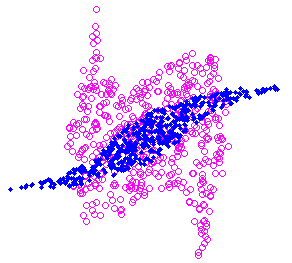
\includegraphics[scale = 0.25]{nonlinear.png}
\end{center} 
\begin{itemize}
\item{One way to approximate a nonlinear independent direction is to use a local linear approximation, which requires an over-complete basis} 
\item{Heuristic requirements for independence: Basis vectors should be sparsely activated}
\end{itemize}
\end{frame} 

\begin{frame}
\small
\frametitle{Relationship Between Approaches} 
\begin{tabular}{c||c|c|c|c}
Algorithm & Model & Encode & Decode & Relate Enc. \& Dec.\\
\hline
\cellcolor{red}PCA & Global Linear &\checkmark & \checkmark & $W_D = W_E ^T$\\
\hline
\cellcolor{red}ICA & Global Linear &\checkmark & \checkmark & $W_D = W_E ^T$\\
\thickhline
\cellcolor{yellow}Sparse Coding & Local Linear &\checkmark(\$) & \checkmark & $W_D = W_E ^T$ \\
\hline 
\cellcolor{yellow}PSD \& LISTA & Local Linear &\checkmark & \checkmark & Learned $W_E$\\
\thickhline
\cellcolor{orange}DrLIM & Nonlinear & \checkmark & X & Enc. Only\\
\hline
\cellcolor{green}Auto-Encoders & Nonlinear & \checkmark & \checkmark & Learned $W_E$ \& $W_D$ 
\end{tabular} \\
\begin{center}
\begin{tabular}{c|c|}
\hline
\cellcolor{red} \hspace{10 mm} & De-correlation/Independence  \\
\cellcolor{yellow} \hspace{10 mm} & Sparsity \\
\hline
\cellcolor{orange} \hspace{10 mm} & Metric Learning/Restricted Metric Learning  \\
\hline
\cellcolor{green} \hspace{10 mm} & All of the Above \\
\hline
\end{tabular}
\end{center} 
\end{frame} 

\begin{frame} 
\begin{center}
\frametitle{Sparse Coding} 
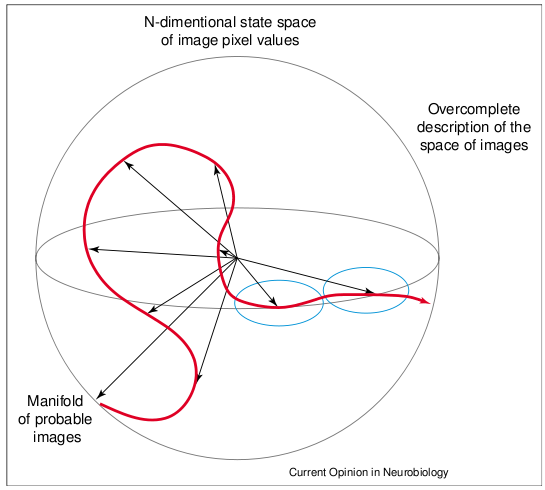
\includegraphics[scale = 0.4]{imageManifold.png} \\
Unlike local PCA, basis elements can be recycled 
\end{center} 
\end{frame} 


\begin{frame}
\frametitle{Sparse Coding}  
\begin{itemize}
\item{Find a sparsely activated over-complete basis which describes the data} 
\item{Direct measure of sparsity, the $L_0$ norm, results in a combinatorial optimization problem} 
\item{Note that another popular measure of sparsity is kurtosis, which links directly back to ICA} 
\item{Modern formulations of sparse coding use the $L_1$ norm as a sparsity measure} 
\begin{eqnarray}
\nonumber
min \| z \| _1 \mbox{ s.t } W z = s \mbox{ (BP)} \\
\nonumber
\min_{z} \frac{1}{2} \|s - W z \|_2 ^2 + \lambda \| z \|_1 \mbox{ (BPDN)} \\ 
\nonumber 
\min_{z, W} \frac{1}{2} \|s - W z \|_2 ^2 + \lambda \| z \|_1 \mbox{ (SC)}
\end{eqnarray} 
\end{itemize} 
\end{frame} 

\begin{frame}
\frametitle{Why $L_1$?}
\begin{center}
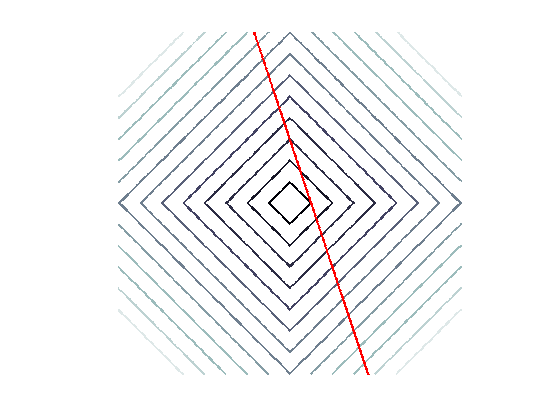
\includegraphics[scale = 0.3]{L1.png} 
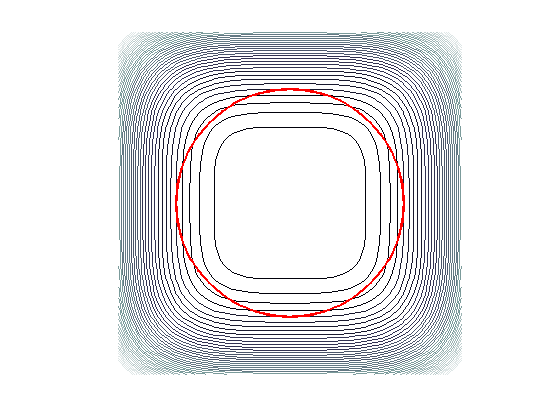
\includegraphics[scale = 0.3]{ICA.png}\\
Left: Minimize $L_1$, goal: sparsity\\ Right: Maximize kurotsis, goal: independence
\end{center} 
\end{frame} 

\begin{frame} 
\frametitle{Implementation} 
\begin{center}
$\min_{z, W} \frac{1}{2} \|s - W z \|_2 ^2 + \lambda \| z \|_1$\\
\begin{itemize}
\item{Alternately optimize $z$ (inference) and $W$ (basis update)}
\item{It is easy to reduce $\|z\|_1$ and increase the norm of the columns of $W$, thus the columns of $W$ must be normalized to unity}
\end{itemize} 
\end{center} 
\end{frame} 

\begin{frame}
\frametitle{ISTA Inference}
\begin{itemize}
\item{Given a fixed basis $W$ there exists a fixed point algorithm for finding the optimal coefficients $z^*$ (i.e. inference)}  
\end{itemize} 
\begin{center} 
$z_{k+1} = shrink(z_k - \eta_1 \nabla_{z_k}\frac{1}{2} \|s - W z_k \|_2 ^2)$
\begin{itemize}
\item{Application of the $shrink()$ function corresponds to a gradient step in $L_1$ }
\end{itemize} 
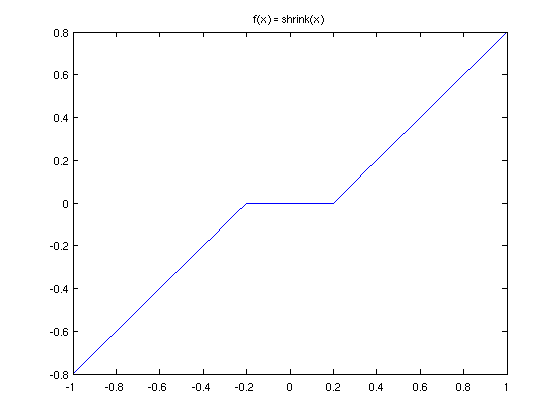
\includegraphics[scale = 0.3]{shrink.png} 
\end{center} 
\end{frame} 

\begin{frame}
\frametitle{LISTA Inference}  
\begin{center} 
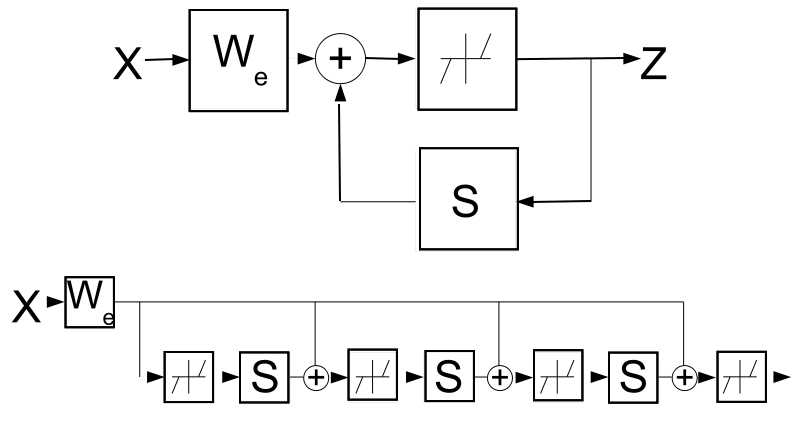
\includegraphics[scale = 0.25]{LISTA.png} \\
$S = I - \frac{1}{L} W_d ^T W_d$ and $W_e = \frac{1}{L} W_d ^T$
\end{center} 
\begin{itemize}
\item{Learned ISTA is a method for approximating the inference step by a feed forward network} 
\item{Since only a finite number of ISTA iterations are performed, $W_e$ and $S$ are trainable} 
\item{Allows the possibility of 'explaining away', unlike PSD}
\end{itemize} 
\end{frame} 

\begin{frame}
\frametitle{Invariance and IPSD}
\begin{itemize}
\item{For a sparse code $\| \frac{\partial z}{\partial x} \|$ can be huge (discontinuous)}  
\item{Invariance is a desired quality, ex: SIFT, HoG} 
\item{Approach: Imposed a topological structure on $z$ by pooling over overlapping neighborhoods, and measure sparsity of the neighborhoods}  
\end{itemize} 
\begin{center}
$\frac{1}{2} \|x - Wz \|_2 ^ 2 + \lambda \sum_{i=1} ^ K \sqrt{\sum_{j \in P_i} w_jz_j ^2}$ 
\begin{itemize} 
\item{$\sqrt{n} < n$ for $n>1$, encourages sparse activations across neighborhoods}
\item{Within neighborhoods $z_j$ are encouraged to co-activate}
\end{itemize}
$\frac{1}{2} \|x - Wz \|_2 ^ 2 + \lambda \sum_{i=1} ^ K \sqrt{\sum_{j \in P_i} w_jz_j ^2} + \alpha \|z - F(x;W) \|_2 ^2$ 
\end{center} 
\end{frame} 

\begin{frame}
\frametitle{Invariance and IPSD}
\begin{center}
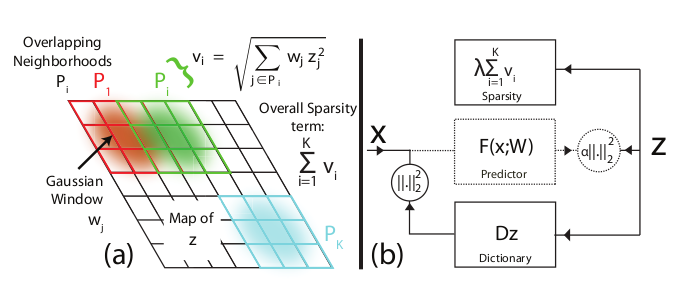
\includegraphics[scale = 0.3]{PSD2.png} \\
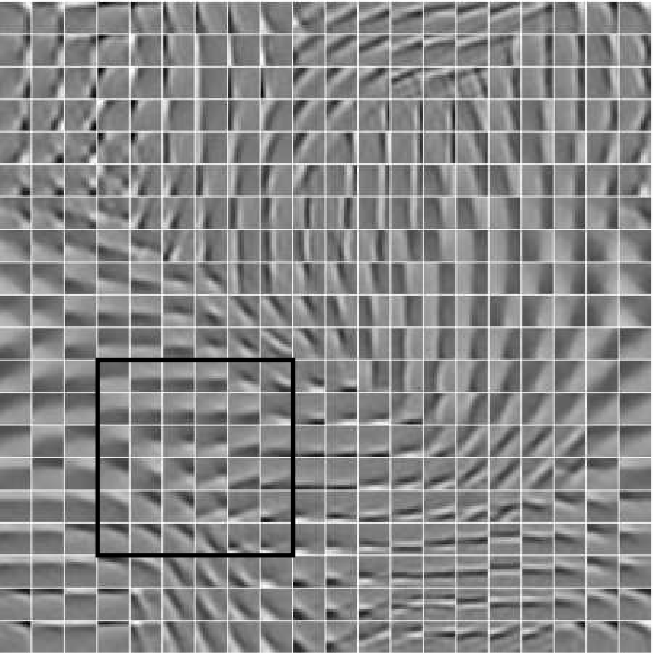
\includegraphics[scale = 0.2]{PSD.png} 
\end{center} 
\end{frame} 

\begin{frame}
\small
\frametitle{Relationship Between Approaches} 
\begin{tabular}{c||c|c|c|c}
Algorithm & Model & Encode & Decode & Relate Enc. \& Dec.\\
\hline
\cellcolor{red}PCA & Global Linear &\checkmark & \checkmark & $W_D = W_E ^T$\\
\hline
\cellcolor{red}ICA & Global Linear &\checkmark & \checkmark & $W_D = W_E ^T$\\
\hline
\cellcolor{yellow}Sparse Coding & Local Linear &\checkmark(\$) & \checkmark & $W_D = W_E ^T$ \\
\hline 
\cellcolor{yellow}PSD \& LISTA & Local Linear &\checkmark & \checkmark & Learned $W_E$\\
\thickhline
\cellcolor{orange}DrLIM & Nonlinear & \checkmark & X & Enc. Only\\
\thickhline
\cellcolor{green}Auto-Encoders & Nonlinear & \checkmark & \checkmark & Learned $W_E$ \& $W_D$ 
\end{tabular} \\
\begin{center}
\begin{tabular}{c|c|}
\hline
\cellcolor{red} \hspace{10 mm} & De-correlation/Independence  \\
\cellcolor{yellow} \hspace{10 mm} & Sparsity \\
\hline
\cellcolor{orange} \hspace{10 mm} & Metric Learning/Restricted Metric Learning  \\
\hline
\cellcolor{green} \hspace{10 mm} & All of the Above \\
\hline
\end{tabular}
\end{center} 
\end{frame} 

\begin{frame}
\frametitle{Metric Learning}  
\begin{itemize}
\item{Geodesic v.s. Euclidean distance}
\item{Another way to pose the problem is to find a distance preserving mapping to lower dimensional space} 
\item{For densely sampled manifolds this makes sense, but for realistic data we are satisfied with preserving some distance metric of interest, possibly mangling others}  
\end{itemize} 
\begin{center} 
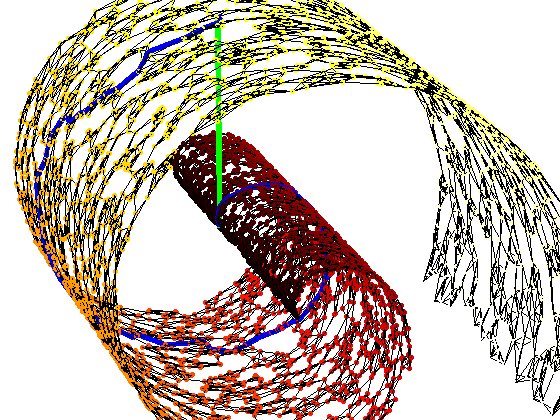
\includegraphics[scale = 0.3]{swiss.png} 
\end{center} 
\end{frame}

\begin{frame}
\frametitle{DrLIM} 
\begin{itemize}
\item{We wish to find a mapping $G_W(X_i): \mathbb{R}^D \rightarrow \mathbb{R}^d$, where $D>d$ which translates labeled similarity relationships in the input space to Euclidean distances in the output space} 
\item{If $(X_1, X_2)$ are similar then $Y=0$, otherwise $Y=1$}
\item{Let $D_W(X_1, X_2) = \|G_W(X_1),G_W(X_2)\|_2$}
\item{$L(W,Y,X_1,X_2) = (1-Y)\frac{1}{2}D_W^2 + Y \frac{1}{2}\{max(0,m-D_W)\}^2$}   
\begin{center}
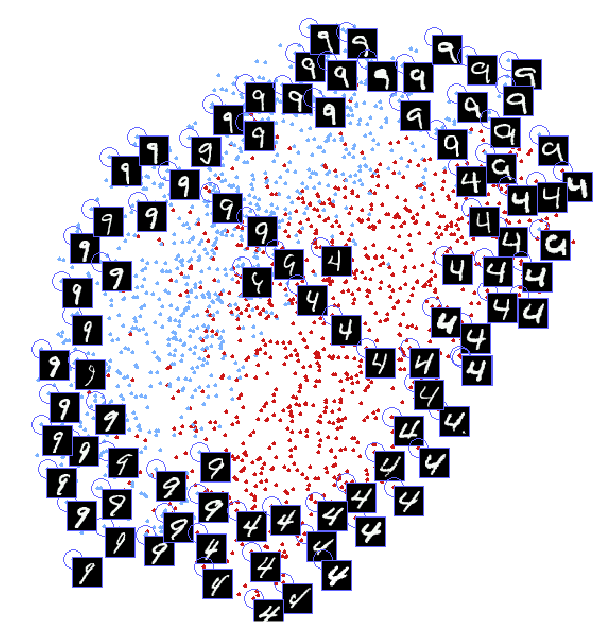
\includegraphics[scale = 0.20]{drlim.png} 
\end{center} 
\end{itemize} 
\end{frame} 

\begin{frame}
\frametitle{DrLIM}
We can do classical metric learning using DrLIM by using $L_2$ as a measure of similarity in the ambient space (n-nearest neighbors)
\begin{center}
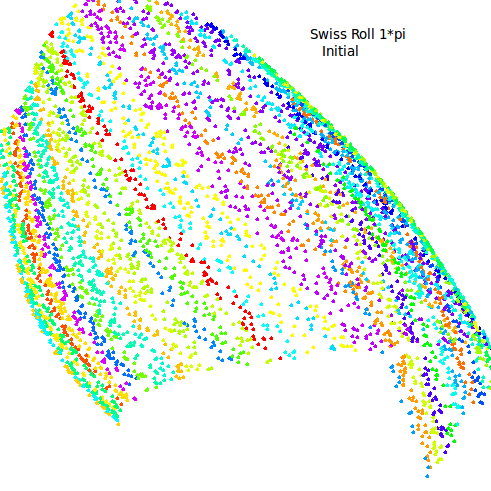
\includegraphics[scale = 0.20]{s1.png} 
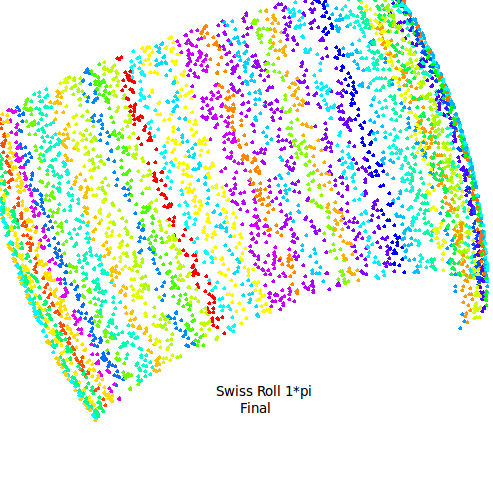
\includegraphics[scale = 0.20]{s2.png} \\
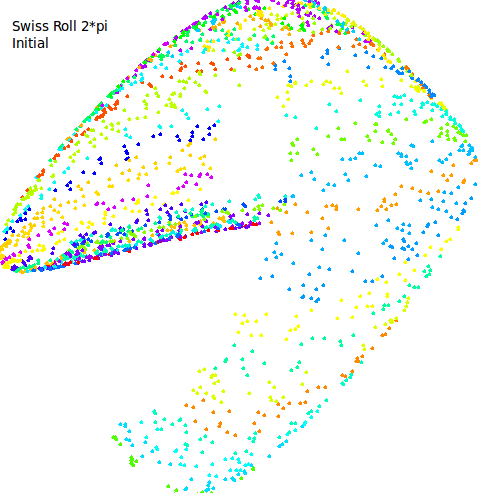
\includegraphics[scale = 0.20]{s3.png} 
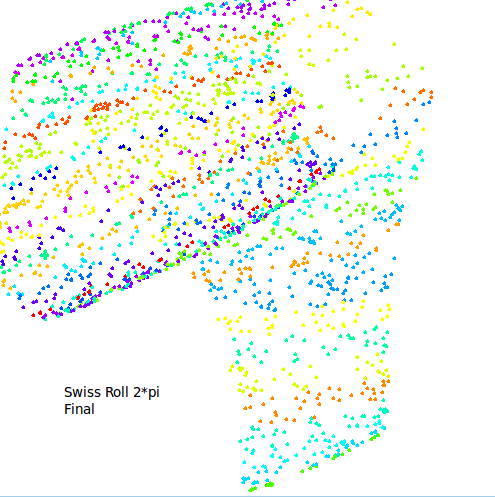
\includegraphics[scale = 0.20]{s4.png} 
\end{center} 
\end{frame} 

\begin{frame}
\small
\frametitle{Relationship Between Approaches} 
\begin{tabular}{c||c|c|c|c}
Algorithm & Model & Encode & Decode & Relate Enc. \& Dec.\\
\hline
\cellcolor{red}PCA & Global Linear &\checkmark & \checkmark & $W_D = W_E ^T$\\
\hline
\cellcolor{red}ICA & Global Linear &\checkmark & \checkmark & $W_D = W_E ^T$\\
\hline
\cellcolor{yellow}Sparse Coding & Local Linear &\checkmark(\$) & \checkmark & $W_D = W_E ^T$ \\
\hline 
\cellcolor{yellow}PSD \& LISTA & Local Linear &\checkmark & \checkmark & Learned $W_E$\\
\hline
\cellcolor{orange}DrLIM & Nonlinear & \checkmark & X & Enc. Only\\
\thickhline
\cellcolor{green}Auto-Encoders & Nonlinear & \checkmark & \checkmark & Learned $W_E$ \& $W_D$ \\
\thickhline
\end{tabular} \\
\begin{center}
\begin{tabular}{c|c|}
\hline
\cellcolor{red} \hspace{10 mm} & De-correlation/Independence  \\
\cellcolor{yellow} \hspace{10 mm} & Sparsity \\
\hline
\cellcolor{orange} \hspace{10 mm} & Metric Learning/Restricted Metric Learning  \\
\hline
\cellcolor{green} \hspace{10 mm} & All of the Above \\
\hline
\end{tabular}
\end{center} 
\end{frame} 

\begin{frame}
\frametitle{Auto-Encoder Framework} 
\begin{itemize}
\item{An Auto-Encoder(AE) is composed of an "encoder" and "decoder"}
\item{The encoder and decoder may correspond to completely different procedures (bases)}
\item{The encoder transforms the data to latent space, and the decoder reconstructs the data from the latent representation}  
\item{AEs unify many data representation concepts and algorithms} 
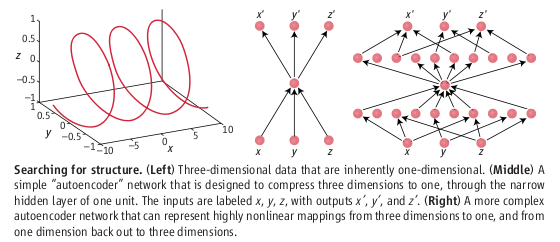
\includegraphics[scale = 0.4]{autoenc.png} 
\end{itemize} 
\end{frame} 

\begin{frame}
\frametitle{Linear AE and PCA} 
\begin{itemize}
\item{Encoding and decoding simply corresponds to multiplication by $W_e$ and $W_d$, respectively}
\item{If $We$ and $Wd$ are full rank, then the AE has the capacity to learn the identity function}  
\item{Using s.g.d the largest eigenvectors of the covariance (or their mixtures) are learned first}
\item{More interesting representations can be hoped for if some nonlinear function is applied to the encoder outputs}
\item{AEs with nonlinearity can be stacked}
\end{itemize}  
\begin{center}
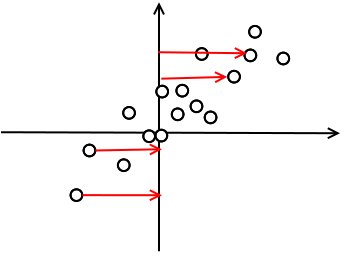
\includegraphics[scale = 0.4]{stochasticPCA.png} 
\end{center} 
\end{frame} 

\begin{frame}
\frametitle{Denoising AE} 
\begin{itemize}
\item{This AE is trained to reconstruct an image from a corrupted version of itself} 
\item{The corruption process randomly chooses some proportion of the pixels in the image and sets them to zero}   
\item{This explicitly forces the AE to learn and exploit dependencies between pixels in images} 
\item{Can be interpreted as simultaneously learning $p(x|\tilde{x})$ and how to infer $x$ from $\tilde{x}$}
\item{If $dim(Y)<dim(X)$ then "$Y=f(X)$ is a representation of $X$ which is well suited for capturing the main variations in the data, i.e. on the manifold"}
\end{itemize} 
\begin{center}
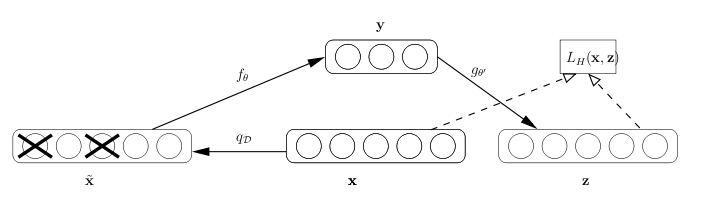
\includegraphics[scale=0.25]{DAE.png}
\end{center} 
\end{frame} 

\begin{frame}
\frametitle{Denoising AE}  
\begin{center}
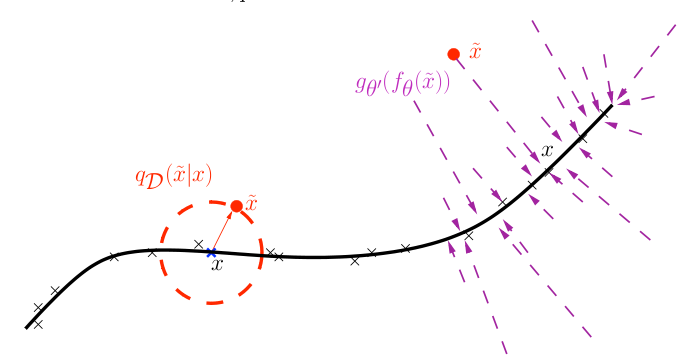
\includegraphics[scale=0.25]{DAE2.png}\\
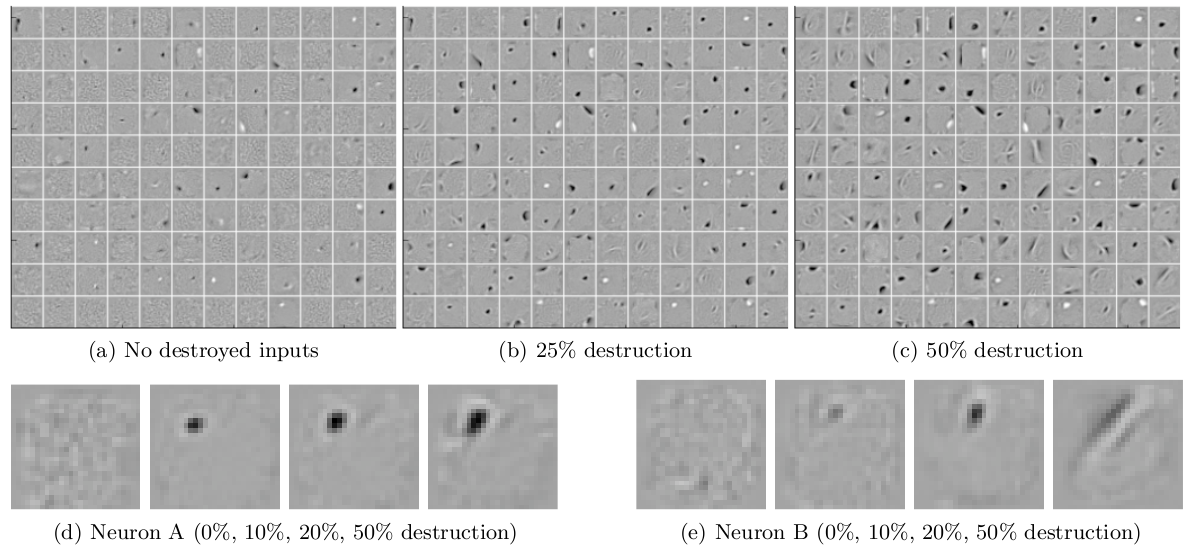
\includegraphics[scale=0.25]{DAE3.png}
\end{center} 
\end{frame} 

\begin{frame} 
\frametitle{Contractive AE}
\begin{itemize}
\item{Other techniques of obtaining "interesting" representations is to regularize the latent representation}
\item{Contrary to more traditional regularization directly on weights, these correspond to "generic prior hypotheses"}
\item{$L_{CAE} = \sum_{x \in D_n} \|x-x_r\|_2 ^2 + \lambda \sum_{ij} \left(\frac{\partial h_j(x)}{\partial x_i} \right)^2$ }
\end{itemize} 
\begin{center}
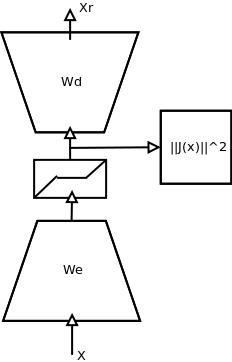
\includegraphics[scale = 0.4]{CAE.png} 
\end{center} 
\end{frame} 

\begin{frame}
\frametitle{Contractive AE} 
\begin{itemize}
\item{$\left(\frac{\partial h_j(x)}{\partial x_i}\right)^2 = (h'_j(x))^2 W_{e_{ij}}^2$}
\item{Important to tie or normalize weights}
\item{If there were no reconstruction objective then the penalty on the Jacobian would produce a constant representation for all inputs either by saturating or weight decay} 
\item{However nearby images on the manifold must be reconstructed as distinct images}
\item{The contractive pressure is counteracted by the reconstruction gradient in the directions tangent to the manifold}
\item{Contractive penalty has a component in the direction of curvature gradient}
\item{Can be interpreted roughly as curvature regularization}
\end{itemize} 
\end{frame} 

\begin{frame}
\frametitle{Relationship with other Auto-Encoders}
\begin{itemize}
\item{Denoising auto-encoders also achieve a contractive mapping of the \emph{reconstruction} via a stochastic process, which indirectly encourages invariance in the latent representation}
\item{Sparse auto-encoders encourage the activations to be zero which occurs in the saturated part of the nonlinearity (assuming a proper choice of nonlinearity, e.g. LISTA)}
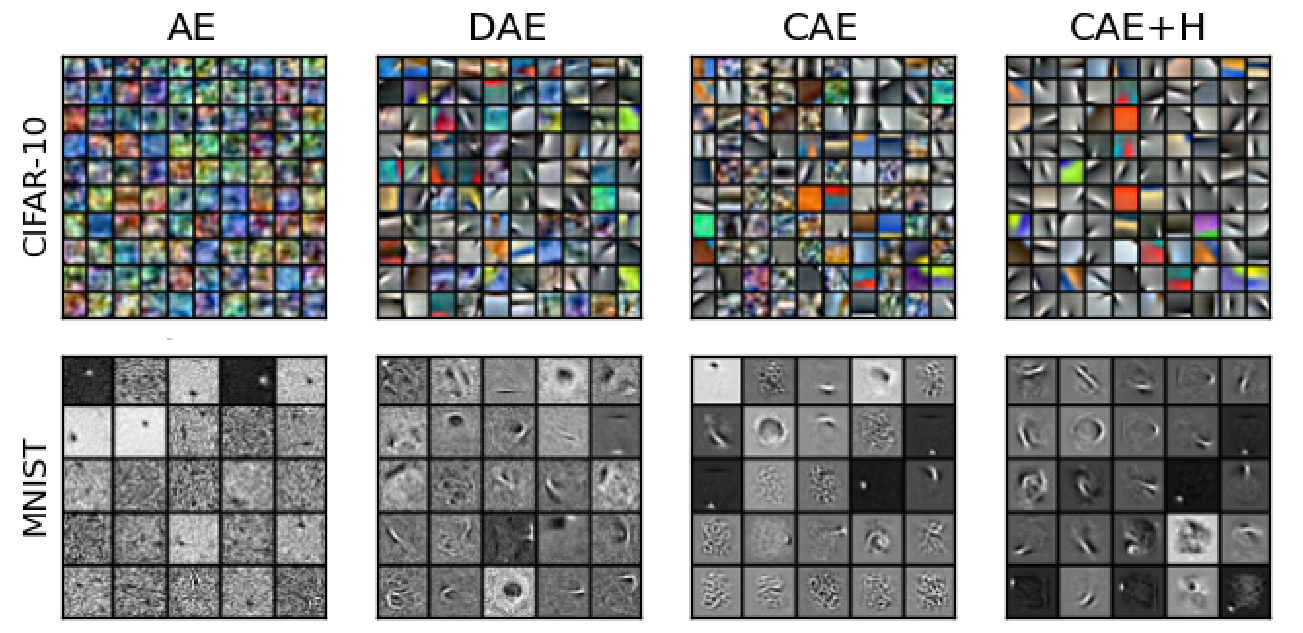
\includegraphics[scale = 0.2]{CAE2.png} 
\end{itemize} 
\end{frame}

\begin{frame}
\frametitle{Saturating Auto-Encoder (SAE)} 
\begin{itemize}
\item{Inspired by the CAE, we introduce a penalty on activations outside the saturated region of the nonlinearity} 
\begin{center}
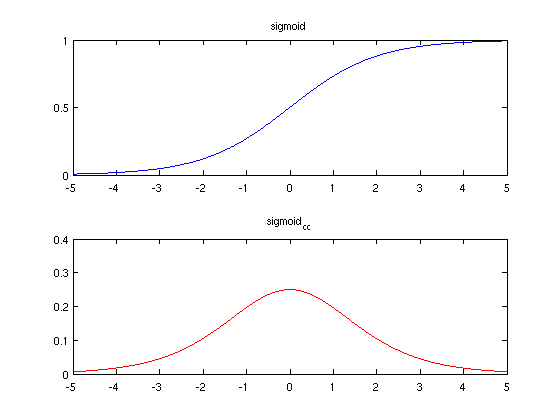
\includegraphics[scale = 0.25]{sigmoid_cc.png}
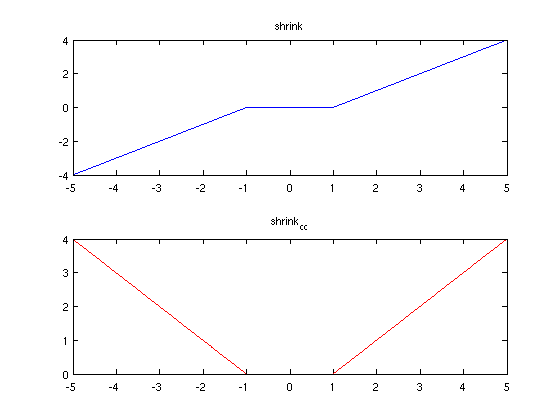
\includegraphics[scale = 0.25]{shrink_cc.png} \\
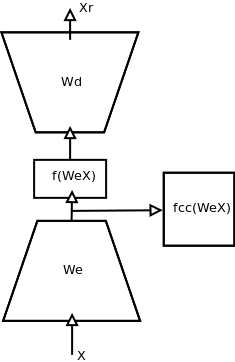
\includegraphics[scale = 0.25]{SAE.png}
\end{center} 
\end{itemize} 
\end{frame} 

\begin{frame} 
\frametitle{SAE with $shrink()$ Nonlinearity} 
\begin{itemize} 
\item{The saturation penalty exactly corresponds to an $L_1$ penalty}
\item{This auto-encoder strongly resembles sparse coding using PSD with $shrink()$ nonlinearity}
\item{Important to enforce $\|w_d\|_2 = 1$ }
\end{itemize} 
\begin{center} 
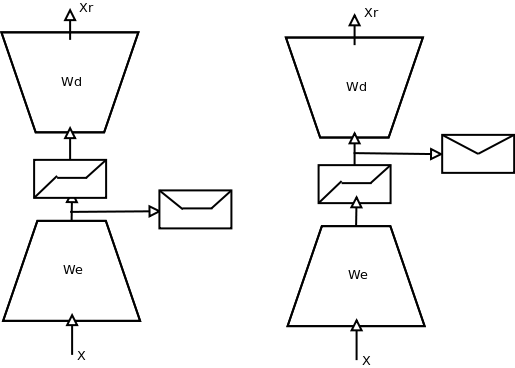
\includegraphics[scale = 0.25]{SAE_shrink.png}
\end{center} 
\end{frame} 

\begin{frame}
\begin{center} 
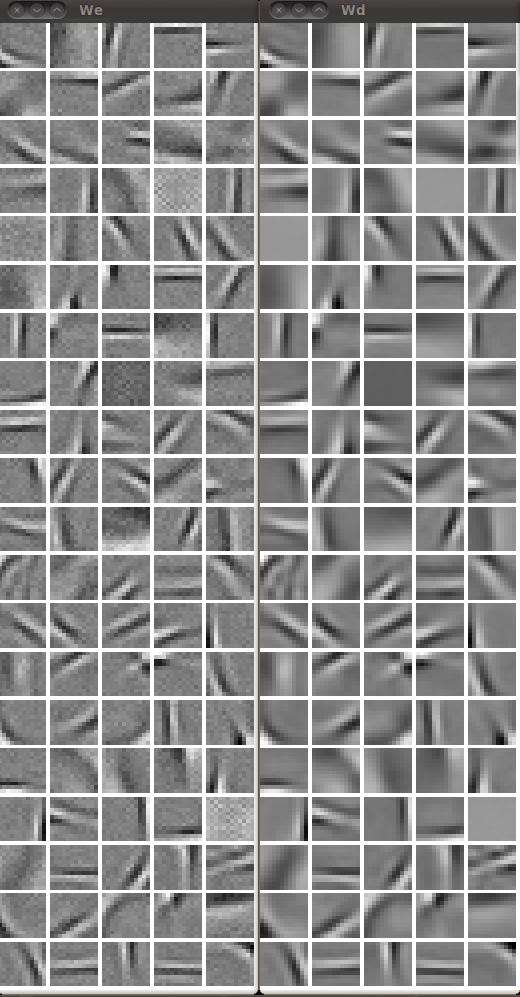
\includegraphics[scale = 0.25]{Wshrink.png}
\end{center} 
\end{frame} 

\begin{frame}
\frametitle{Geometric Interpretation} 
\begin{itemize}
\item{Assume all the data points (circles) and decoder bases (arrow) are normalized to unity}
\item{$\frac{\partial E_{rec}}{\partial W_d} = (x-x_{rec})shrink(W_ex)^T$}  
\item{The $shrink()$ function explicitly promotes locality (specialization) of the basis elements by restricting the range of influence to nearby data points}
\end{itemize} 
\begin{center}
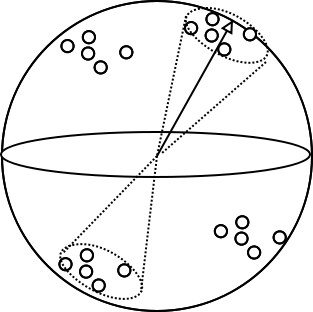
\includegraphics[scale = 0.40]{shrink_geom.png}  
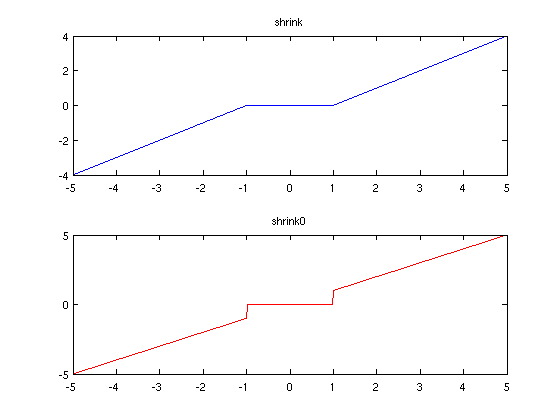
\includegraphics[scale = 0.25]{shrink0.png}  
\end{center} 
\end{frame}

\begin{frame} 
\frametitle{Interpretation of Nonlinearities} 

\end{frame} 

\begin{frame}
\frametitle{Enforcing a Factorization: Transforming Auto-Encoders} 
\begin{itemize}
\item{"Move to a space in which the common variabilities can be described by linear transformations" (Hinton, 2012)}
\item{In the case of objects in images: A representation in which the identity of the object (what?)  is separately represented from the configuration (where?) would satisfy the above requirement}
\item{This corresponds to a physically interpretable latent representation}
\end{itemize} 
\end{frame} 

\begin{frame}
\frametitle{Enforcing a Factorization: Transforming Auto-Encoders} 
\begin{center}
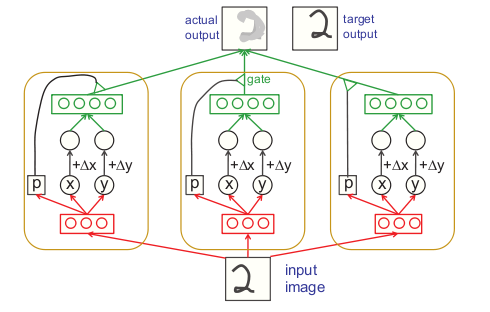
\includegraphics[scale = 0.4]{capsules.png}
\end{center}
Each capsule has the capacity to represent only one instance of its visual entity at a time
\end{frame}

\begin{frame}
\frametitle{Inverting Auto-Encoder}
\begin{itemize}
\item{$R_W(G(y_i')) = y_i''$ if $R_W = G^{-1}$ then $y_i' = y_i''$ thus we want to $min_W \|y_i'-y_i''\|$} 
\end{itemize} 
\begin{center}
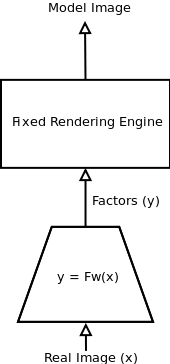
\includegraphics[scale = 0.4]{render.png}
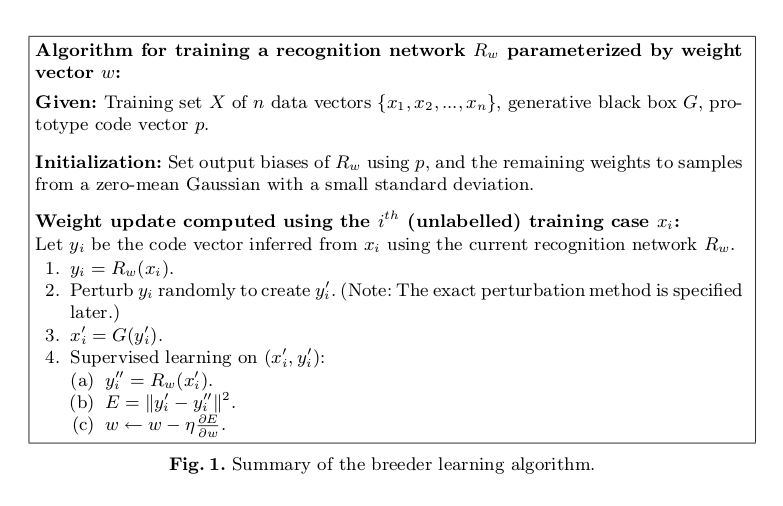
\includegraphics[scale = 0.25]{alg.png}
\end{center}
\end{frame} 

\begin{frame}
\frametitle{Inverting Auto-Encoder}
\begin{center}
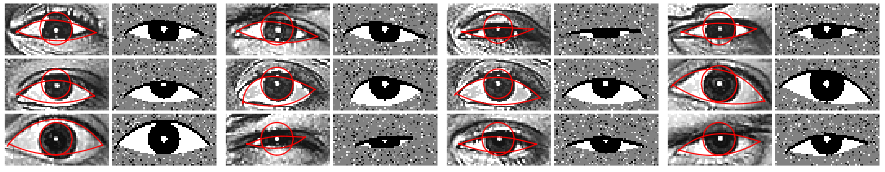
\includegraphics[scale = 0.3]{eyes.png}\\
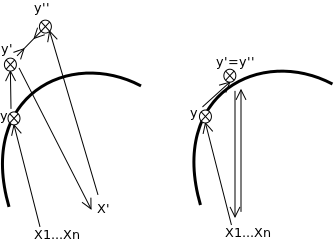
\includegraphics[scale = 0.3]{breeder.png}
\end{center} 
\end{frame} 

\begin{frame}
\centerline{
\huge
\emph{Thank You}} 
\vspace{10 mm} 
\centerline{
\huge
\emph{THE END}} 

\end{frame}

\end{document}


